\chapter{Progettazione e implementazione}
\label{cap:progettazione-codifica}

\lstset{
    escapeinside={(*@}{@*)}, % Delimitatori per modalità LaTeX
    basicstyle=\ttfamily,    % Stile monospaziato
}

\intro{Questo capitolo è incentrato sulla progettazione e sulla codifica dell'algoritmo, mostrando passo per passo il suo funzionamento}


\section{Progettazione}

Questa sezione esplora i diversi aspetti fondamentali nella progettazione di un algoritmo genetico: le componenti fondamentali, la struttura e gli operatori genetici.

\subsection{Composizione degli algoritmi evolutivi}

I principali componenti di ricerca per progettare un algoritmo evolutivo sono i seguenti:

\begin{itemize}
    \item \textbf{Rappresentazione}: negli algoritmi genetici, la soluzione codificata è chiamata cromosoma, mentre le variabili decisionali all'interno di una soluzione (cromosoma) sono i geni;
    
    \item \textbf{Inizializzazione della popolazione}: la generazione della popolazione iniziale è un aspetto cruciale in quanto una giusta inizializzazione determina un vantaggio già dalle prime interazioni;
    
    \item \textbf{Funzione di fitness}: si tratta della funzione obbiettivo, ogni soluzione ha un valore di fitness che indica il grado di adeguatezza rispetto al problema;
    
    \item \textbf{Strategia di selezione}: la strategia di selezione affronta la seguente domanda: "Quali genitori per la prossima generazione vengono scelti con un bias verso un fitness migliore?";
    
    \item \textbf{Strategia di riproduzione}: la strategia di riproduzione consiste nel progettare operatori di mutazione e crossover adeguati per generare nuovi individui (discendenti);
    
    \item \textbf{Strategia di sostituzione}: i nuovi discendenti competono con gli individui più vecchi per ottenere il loro posto nella prossima generazione (sopravvivenza del più adatto);
    
    \item \textbf{Criteri di arresto}: determina la fine del loop evolutivo, solitamente è indicato come il numero di generazioni da raggiungere, ovvero ogni interazione è una generazione.
\end{itemize}

\subsection{Struttura del genetico}

In questa sezione descriviamo la struttura dell'Algoritmo Genetico scelta per il controllo delle sue fasi di intensificazione e diversificazione.
L'obiettivo è massimizzare una funzione di fitness $f$. I parametri richiesti dall'algoritmo GA sono:

\begin{itemize}
    \item $N$: dimensione della popolazione;
    \item $p_c$: probabilità di crossover;
    \item $p_m$: probabilità di mutazione;
    \item $M$: dimensione del pool di accoppiamento;
    \item $E$: dimensione dell'élite.
\end{itemize}

Indichiamo con $P$ la popolazione di cromosomi e con $G$ l'insieme di discendenti generati dalla fase di riproduzione.

\begin{lstlisting}
def GA(N, pc, pm, M, E):
    P = generate(N);
    while not terminate() do
        G = reproduction(P, pc, pm, M);
        P = replace(P, G, E);
    end
    return maxf P;
end
\end{lstlisting}

\subsubsection{Riproduzione}
In questa fase utilizziamo operatori binari (crossover) e unari (mutazione) per esplorare altre soluzioni alterando solo una parte della soluzione. Questa modifica parziale (invece di una riorganizzazione totale, che sarebbe una ricerca casuale), insieme al sostegno degli individui più idonei (es. selezione dei genitori), porta l'algoritmo a spingere avanti nelle generazioni le soluzioni più idonee mantenendo un buon tasso di esplorazione di nuovi cromosomi. La dimensione dei discendenti richiesta è pari alla dimensione della popolazione $N$, che poi subisce la procedura di sostituzione.

La probabilità di riproduzione indicata con $Be(p)$, ovvero, la variabile casuale di Bernoulli che assume valore 1 con probabilità $p$ e 0 con probabilità $1-p$.

\begin{lstlisting}
    def Reproduction(P, pc, pm, M):
        G = [ ];
        pool = sortf(P)[0 : M];
        while not |G| == |P| do
            par1, par2 = selection(pool);
            if Be(pc) == 1 then
                c1, c2 = crossover(par1, par2);
            else
                c1, c2 = par1, par2;
            end
            G = G (*@$\cup$@*) {c1, c2};
        end
        foreach g (*@$\in$@*) G do
            if Be(pm) == 1 then
                mutation(c);
            end
        end
        return G;
    end
\end{lstlisting}

\subsubsection{Rimpiazzo}
La strategia di rimpiazzo ha un grande impatto sull'intensificazione. La metodologia di rimpiazzo adottata può essere spiegata in due passaggi: 
\begin{enumerate}
    \item i migliori $E$ elementi nell'unione di $P$ e $G$ fanno automaticamente parte della popolazione successiva;
    \item i migliori $|P| - E$ discendenti di $G$ sono inclusi nella popolazione successiva.
\end{enumerate}

\begin{lstlisting}
    def Replace(P, G, E):
        elite = best subset(P (*@$\cup$@*) G, E, f);
        Gbest = best subset(G, |P| - E, f);
        return elite (*@$\cup$@*) Gbest;
    end
\end{lstlisting}

\subsection{Operatori genetici}

Gli operatori genetici permettono agli algoritmi evolutivi di modulare la diversificazione. Operano sui cromosomi alterandone i geni e permettendo di esplorare un ampio spazio di soluzioni senza andare a perdere intensificazione grazie alla selezione e all'elitismo.

\subsubsection{Selezione}

La selezione dei genitori viene effettuata sui migliori \( M \) individui della popolazione attuale, i quali costituiscono il cosiddetto \emph{Mating Pool}.

Il meccanismo di selezione è uno dei principali componenti di ricerca negli algoritmi evolutivi (EAs). Il principio fondamentale dei metodi di selezione è: \emph{"più un individuo è valido, maggiore è la sua probabilità di essere scelto come genitore."} Questa pressione selettiva guida la popolazione verso soluzioni migliori. Tuttavia, gli individui peggiori non dovrebbero essere completamente scartati, poiché essi potrebbero contenere materiale genetico utile.

La strategia di selezione determina quali individui vengono scelti per l'accoppiamento (riproduzione).

La selezione tramite ruota della roulette è la strategia di selezione più comune. Essa assegna a ciascun individuo una probabilità di selezione proporzionale alla sua fitness relativa. Sia $f_i$ la fitness dell'individuo $p_i$ nella popolazione $P$. La probabilità di selezione è data da:

\[ p_i = \frac{f_i}{\sum_{j=1}^{n} f_j} \]

Immaginiamo un grafico a torta in cui a ciascun individuo è assegnato uno spazio proporzionale alla sua fitness. Una ruota della roulette è posizionata attorno al grafico. La selezione di $\mu$ individui avviene tramite $\mu$ spin indipendenti della ruota. Ogni spin seleziona un singolo individuo. Gli individui migliori occupano più spazio e, di conseguenza, hanno maggiori probabilità di essere scelti (Figura 5.2).

\begin{figure}[!ht] 
    \centering 
    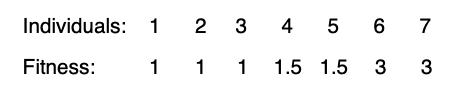
\includegraphics[width=0.6\columnwidth]{tesi/fitness_roulette_wheel} 
    \caption{Pesi della ruota}
\end{figure}

\begin{figure}[!ht] 
    \centering 
    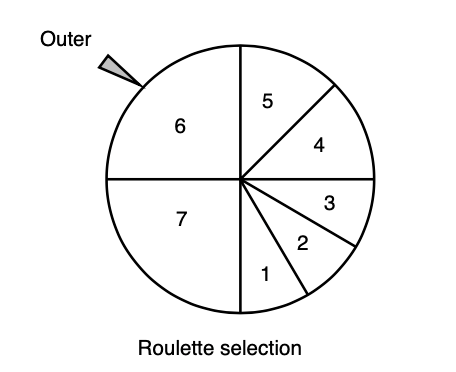
\includegraphics[width=0.6\columnwidth]{tesi/roulette_wheel} 
    \caption{Grafico a torta della selezione tramite ruota della roulette}
\end{figure}

Tuttavia, nella selezione tramite ruota della roulette, individui eccezionali possono introdurre un bias all'inizio della ricerca, causando una convergenza prematura e una perdita di diversità genetica. Infatti, va notato che un valore di \( M \) troppo piccolo intensifica il focus sui migliori individui del \emph{Mating Pool}, riducendo però la diversificazione della popolazione. Questo compromesso deve essere attentamente bilanciato per garantire un efficace equilibrio tra esplorazione e sfruttamento nel processo evolutivo.

\subsubsection{Crossover}
Il crossover prende i due genitori selezionati e genera due figli da aggiungere ai nuovi discendenti. Un crossover avviene con una probabilità $p_c$, altrimenti i genitori vengono semplicemente clonati e aggiunti ai discendenti. L'operatore di crossover, da un lato, mescola i geni delle coppie di cromosomi esplorando nuove soluzioni; dall'altro, se la diversità genetica (individui diversi) nella popolazione è bassa, può portare a una convergenza prematura. Nel caso estremo in cui abbiamo una popolazione composta da elementi tutti uguali, il crossover non può creare nuovi individui. Per garantire la diversità genetica, si può ridurre la fase di intensificazione (es. $E$ o $M$) o aumentare il tasso di mutazione $p_m$.

A differenza degli operatori unari, come la mutazione, l'operatore di crossover è binario e talvolta n-ario. Il ruolo degli operatori di crossover è di ereditare alcune caratteristiche dei due genitori per generare i discendenti. Come per l'operatore di mutazione, la progettazione degli operatori di crossover dipende principalmente dalla rappresentazione utilizzata.

Applicare operatori di crossover classici alle permutazioni, come nel nostro caso, genera soluzioni che non sono permutazioni (ossia, soluzioni non valide). Di conseguenza, sono stati progettati numerosi operatori di crossover per permutazioni, tra cui il crossover a ordine (OX). Per prima cosa, due punti di crossover vengono selezionati casualmente. Dal genitore 1, si copia nel discendente, alle stesse posizioni assolute, la parte tra i due punti. Dal genitore 2, si parte dal secondo punto di crossover e si scelgono gli elementi non già selezionati dal genitore 1, inserendoli nel discendente a partire dal secondo punto di crossover. L'operatore di crossover OX è un operatore di pura ricombinazione. Se si inizia a riempire o scegliere dal primo punto di crossover, l'operatore non sarà puro. Dal genitore 1, vengono preservati l'ordine relativo, l'adiacenza e le posizioni assolute. Dal genitore 2, viene preservato solo l'ordine relativo.

\begin{figure}[!ht] 
    \centering 
    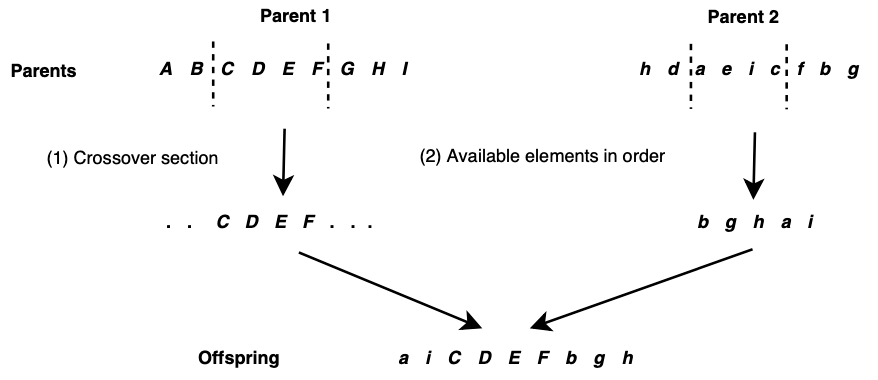
\includegraphics[width=1\columnwidth]{tesi/OXCrossover} 
    \caption{Rappresentazione del crossover OX}
\end{figure}

\subsubsection{Mutazione}
La mutazione viene eseguita dopo il crossover e crea una perturbazione casuale del cromosoma selezionato. Il ruolo della mutazione è duplice: da un lato, simile all'operatore di crossover, provoca una perturbazione di una soluzione per favorire l'esplorazione; dall'altro aumenta la diversità genetica anche se l'attuale diversità è scarsa. Questo è in contrasto con il crossover, che non può diversificare molto un set di individui molto simili.

Gli operatori di mutazione sono operatori unari che agiscono su un singolo individuo. Le mutazioni rappresentano piccoli cambiamenti degli individui selezionati nella popolazione. La probabilità $p_m$ definisce la probabilità di mutare ogni elemento (gene) della rappresentazione. Alcune strategie inizializzano la probabilità di mutazione a $1/k$, dove $k$ è il numero di variabili decisionali, in modo che in media solo poche variabili vengano mutate.

Alcuni punti importanti da considerare nella progettazione o nell'uso di un operatore di mutazione sono i seguenti:

\begin{itemize}
    \item \textbf{Ergodicità}: l'operatore di mutazione dovrebbe consentire di raggiungere ogni soluzione nello spazio di ricerca.
    \item \textbf{Validità}: l'operatore di mutazione dovrebbe produrre soluzioni valide. Questo non è sempre possibile nei problemi di ottimizzazione vincolati.
    \item \textbf{Località}: la mutazione dovrebbe produrre un cambiamento minimo. La dimensione della mutazione è importante e dovrebbe essere controllabile. La località è l'effetto sulla soluzione (fenotipo) quando si esegue la modifica (perturbazione) nella rappresentazione (genotipo). Quando vengono effettuati piccoli cambiamenti nel genotipo, il fenotipo deve rivelare piccoli cambiamenti. In questo caso, si dice che la mutazione ha una forte località. Una debole località è caratterizzata da un grande effetto sul fenotipo quando viene effettuato un piccolo cambiamento nel genotipo.
\end{itemize}

La mutazione in rappresentazioni basate sull'ordine, come nel nostro caso, è generalmente basata sugli operatori di scambio (swapping), inversione o inserimento. 

\section{Parametrizzazione}

In questa sezione viene discussa e motivata la scelta dei valori dei parametri dell'algoritmo tenendo contro delle caratteristiche da ottimizzare, delle istanze di prova fornite dall'azienda e di possibili rischi di overtuning.

L'obbiettivo è quello scegliere una configurazione ottimale di parametri dell'algoritmo per cercare di ottimizzare le seguenti caratteristiche:
\begin{itemize}
	\item\textbf{Intensificazione}: ci si aspetta che il valore di fitness della soluzione migliore all'interno della popolazione incrementi nel corso delle generazioni;
	\item\textbf{Diversificazione}: l'algoritmo deve esplorare un vasto insieme di soluzioni, gli operatori di crossover e mutazione potranno generare soluzioni con valori fitness inferiori a quello della peggiore soluzione della generazione precedente. Quando questo avviene significa che l'algoritmo sta esplorando anche soluzioni diverse, tuttavia non è necessariamente indice che l'esplorazione avvenga in maniera sufficente;
	\item\textbf{Costo computazionale}: come vedremmo in seguito, il criterio di arresto dei test svolti sull'algoritmo è un limite di tempo impostato a 30 secondi. In base all'istanza, è possibile che in 30 secondi vengano computizzate 10 o 100 generazioni. Siccome gli algoritmi genetici sono progettati per funzionare al meglio con l'incrementarsi di generazioni, il limite di tempo non è un criterio di arresto ottimale, tuttavia è necessario per confronti o test. Questo rende la velocità di esecuzione un aspetto di cui tenere conto per permettere all'algoritmo di eseguire più generazioni possibili nel tempo limite.
\end{itemize}

\subsection{Scelta delle configurazioni}

I parametri da configurare sono:
\begin{itemize}
	\item\textbf{population\_size}: dimensione della popolazione di cromosomi, ovvero le soluzioni sul quale lavora il genetico;
	\item\textbf{crossover\_prob}: probabilità che l'algoritmo svolga l'operazione di crossover (applicata a coppie di soluzioni presenti nella pool);
	\item\textbf{mutation\_prob}: probabilità che l'algoritmo svolga l'operazione di mutazione (applicata a ogni soluzione presente nella pool);
	\item\textbf{mating\_pool\_size}: dimensione del pool di accoppiamento;
	\item\textbf{elite\_size}: dimensione dell'insieme dei migliori cromosomi della popolazione che verranno inseriti direttamente nella popolazione della generazione successiva.
\end{itemize}

\noindent La configurazione iniziale (fornita dal tutor aziendale sulla base risultati ottenuti per un algoritmo genetico svolto su un altro problema) è, \textbf{Conf1}:
\begin{itemize}
	\item\textbf{population\_size}: 50;
	\item\textbf{crossover\_prob}: 0,7 (70\%);
	\item\textbf{mutation\_prob}: 0,3 (30\%);
	\item\textbf{mating\_pool\_size}: 20;
	\item\textbf{elite\_size}: 5.
\end{itemize}

Di seguito verranno mostrati alcuni grafici di test svolti su delle singole istanze di prova, fornite appositamente dall'azienda, allo scopo di mostrare l'andamento del valore di fitsess delle soluzioni della determinata istanza. Inoltre, per i test sui parametri dell'algoritmo è stato imposto un criterio di arresto non a limite di tempo ma a limite di generazioni, ed è stato fissato a 50 generazioni. 
L'asse y rappresenta il valore di fitness (da 0.75 a 0.95, dove 0 significa che lo spazio sprecato è tutto, e 1 che non c'è spazio sprecato). L'asse x rappresenta il numero di generazioni (da 0 a 50).
La trasparenza è regolata in modo che più sono presenti cromosomi maggiore è l'intensità del blu.

Dal seguente grafico (Figura 5.4) si nota come ci sia una buona diversificazione ma il valore di fitness della soluzione migliore converge troppo presto, infatti, intorno alla 15esima generazione stabilizza il valore di fitness della soluzione migliore. 

\begin{figure}[!ht] 
    \centering 
    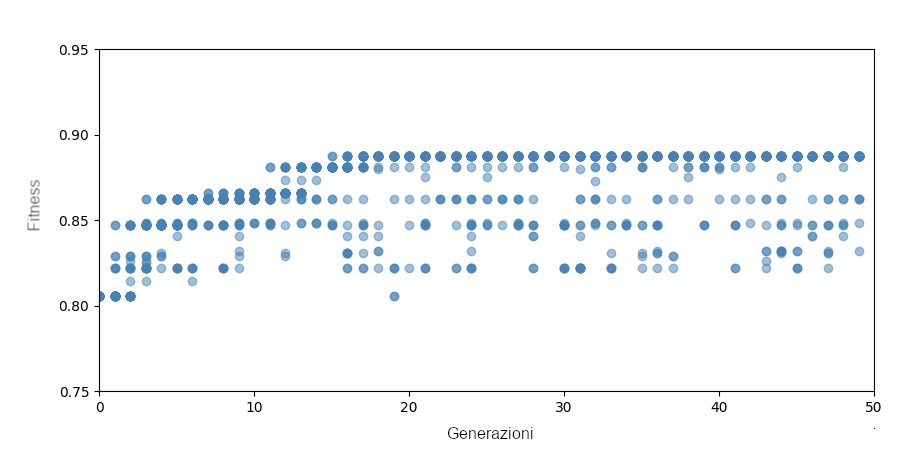
\includegraphics[width=1\columnwidth]{tesi/conf1} 
    \caption{Andamento valori di fitness di un instanza di prova testata con Conf1}
\end{figure}

\textbf{Conf2}:
\begin{itemize}
	\item\textbf{population\_size}: 50;
	\item\textbf{crossover\_prob}: 0,7 (70\%);
	\item\textbf{mutation\_prob}: 0,3 (30\%);
	\item\textbf{mating\_pool\_size}: 40;
	\item\textbf{elite\_size}: 5.
\end{itemize}

Per cercare subito un confronto la prima modifica è stata nella \emph{mating\_pool\_size}, portandola a 40 (da 20) (Figura 5.5), questo ha aumentato notevolmente la diversificazione ed ha trovato soluzioni con un valore di fitness migliore delle soluzioni migliori con la Conf1. 

\begin{figure}[!ht] 
    \centering 
    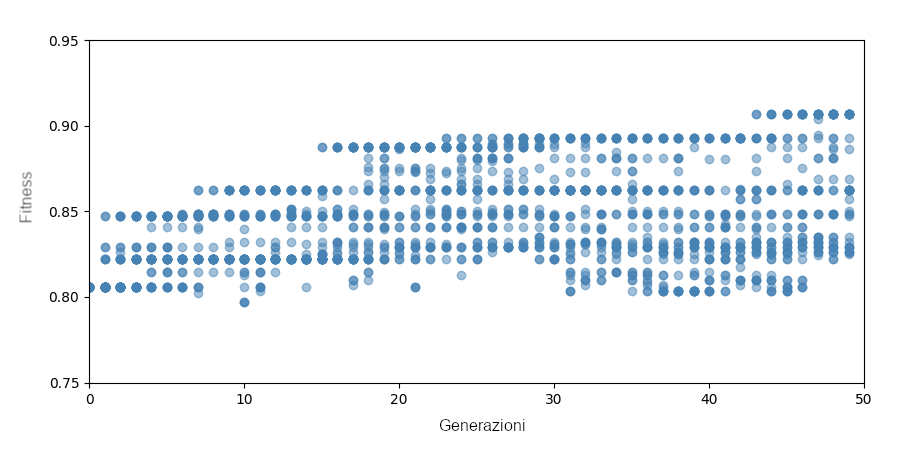
\includegraphics[width=1\columnwidth]{tesi/conf2} 
    \caption{Andamento valori di fitness di un instanza di prova testata con Conf2}
\end{figure}

Questo ha indicato come sicuramente sono presenti soluzioni migliori ottenibili con lo stesso numero di generazioni. Come si può notare, la Conf2 ha molta diversificazione, quindi l'obbiettivo di una nuova configurazione era migliorare l'intensificazione e cercare di diminuire la diversificazione senza perdere le nuove soluzioni che hanno ottenuto un valore di fitness migliore. Si è provato a diminuire la \emph{mating\_pool\_size} e aumentare la \emph{elite\_size} per aumentare l'intensificazione, ma è stato chiaro da subito che un 10\% di \emph{elite\_size} era già il massimo ottenibile senza ridurre drasticamente la diversificazione. Quindi si è provato ad aumentare \emph{crossover\_prob} ma con scarso successo. Sono state tentate anche configurazioni con diverse \emph{mutation\_prob} ma diminuendola si notava chiaramente un appiettimento della diversificazione, mentre, non si rendeva necessario aumentarla dato che un aumento della \emph{mating\_pool\_size} è sufficente per ottenere un giusto livello di diversificazione e aumenta anche l'intensificazione grazie al crossover.

\noindent L'equilibrio è stato trovato con la \textbf{Conf3}:
\begin{itemize}
	\item\textbf{population\_size}: 50;
	\item\textbf{crossover\_prob}: 0,7 (70\%);
	\item\textbf{mutation\_prob}: 0,3 (30\%);
	\item\textbf{mating\_pool\_size}: 30;
	\item\textbf{elite\_size}: 5.
\end{itemize}

(Figura 5.6), una \emph{mating\_pool\_size} corrispondente al 60\% della popolazione, ha generato un bilanciamento ottimale fra intensificazione, diversificazione e velocità di esecuzione. Infatti un altro problema della Conf2, era che una \emph{mating\_pool\_size} di 40 faceva svolgere una generazione in molto più tempo rispetto alla Conf1, quindi, essendo che i test di confronto con la soluzione aziendale, sarebbero stati svolti non con un criterio di arresto basato sulle generazione ma sul tempo, è stato necessario diminuire la \emph{mating\_pool\_size}.

\begin{figure}[!ht] 
    \centering 
    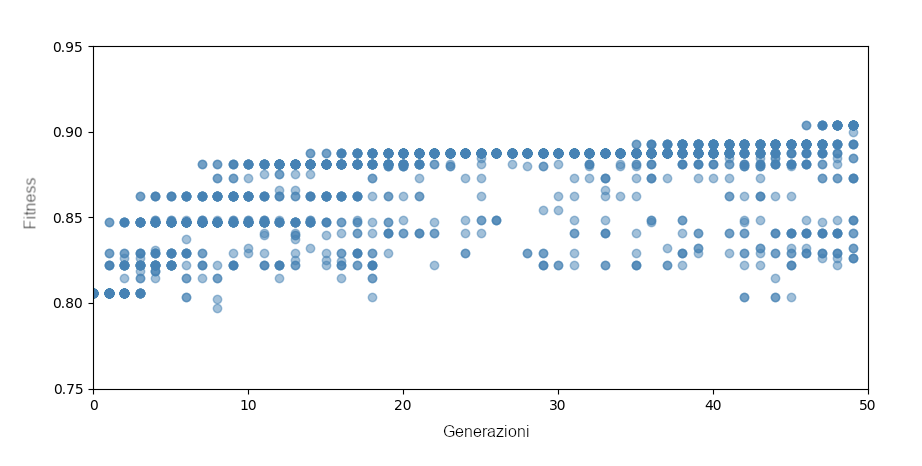
\includegraphics[width=1\columnwidth]{tesi/conf3} 
    \caption{Andamento valori di fitness di un instanza di prova testata con Conf3}
\end{figure}

\subsection{Analisi statistica}

50 istanze di prova diverse generate randomicamente, ciascusa istanza ha:
\begin{itemize}
	\item 1 solo tipo di foglio;
	\item 20 item obbligatori più 0 o 6 o 12 item opzionali;
	\item 0 o metà o tutti gli item obbligatori di una classe hanno margini;
	\item 0 o 20 precedenze, ovvero o nessun item obbligatorio ha precedenze oppure tutti gli obbligatori hanno una precedenza diversa.
\end{itemize}

Le seguenti medie sono ottenute sui valori di fitness della soluzione miglire, per ogni istanza, e il tempo (in secondi) impiegato per eseguire le 50 generazioni.

\begin{itemize}
    \item \textbf{Conf1}
    \begin{itemize}
        \item\textbf{Fitness}: 0.7785907496795459
        \item\textbf{Tempo}: 26.64 
    \end{itemize}
    \item \textbf{Conf2}
    \begin{itemize}
        \item\textbf{Fitness}: 0.7804101596824722
        \item\textbf{Tempo}: 27.76
    \end{itemize}
    \item \textbf{Conf3}
    \begin{itemize}
        \item\textbf{Fitness}: 0.780764190701669
        \item\textbf{Tempo}: 27.26
    \end{itemize}
\end{itemize}

Si può notare che da questi risultati si ottiene una configurazione migliore, tuttavia di tratta solo di risultati basati su determinate istanze. È importante sottolineare che tramite un t-test non sono stati rilevati sufficenti risultati per affermare che a livello statistico una configurazione è migliore di un altra. 

\section{Implementazione}

Di seguto viene decritto il processo implementativo. In particolare la classe \emph{GA} che modella l'algoritmo genetico e \emph{Chromosome} che facilita la manipolazione dei cromosomi all'interno di \emph{GA}.

Per rendere il codice più pulito, mantenibile e comprensibile, sono state usate le linee guida espresse in \textbf{Clean Code}

\subsection{Classe \emph{chromosome}}

La classe \emph{Chromosome} modella un cromosoma, ovvero una possibile soluzione, in una struttura dati che incapsula una sequenza di geni (ovvero gli \emph{Item}, o elementi) e il relativo valore di fitness, grado di adeguatezza del cromosoma al problema. La classe è progettata per essere versatile, con metodi che facilitano la manipolazione e l'evoluzione di cromosomi durante l'esecuzione dell'algoritmo.

La classe \textbf{Item} rappresenta un elemento \( i \in E_O\) o \( j \in E_P\) posizionabile su un foglio \( t \in T \). Ogni elemento è caratterizzato da un identificativo univoco e da un tipo che ne determina proprietà fisiche come larghezza, altezza, margini e altre specifiche geometriche.

Le dimensioni e la posizione dell'oggetto sono definite da attributi come larghezza, altezza, la coordinata del punto superiore sinistro, e l'angolo di rotazione, che può assumere valori predefiniti ( 0°, 90°, 180°, 270°). Vengono calcolate dinamicamente proprietà come area e perimetro, utili per ottimizzazioni, e sono gestite le rotazioni consentite per ogni oggetto. Inoltre, include vincoli di precedenza, sia \emph{hard} che \emph{soft}, che regolano l'ordine in cui può essere posizionato.

\subsubsection*{Attributi}

\begin{itemize}
    \item \textbf{\texttt{genes}}:
    \begin{itemize}
        \item \textbf{Tipo}: Lista
        \item \textbf{Descrizione}: Contiene la sequenza di geni che rappresenta la soluzione codificata. I geni vengono costruiti all'inizio del processo di generazione della popolazione iniziale all'interno del genetico, utilizzando i parametri di input \emph{items} e \emph{optionals}, che corrispondono agli elementi obbligatori \( E_O \) e opzionali \( E_P \) di un istanza. \emph{items} e \emph{optionals} sono codificati come una sequenza \emph{Item}.
    \end{itemize}
    \item \textbf{\texttt{fitness}}:
    \begin{itemize}
        \item \textbf{Tipo}: Float
        \item \textbf{Descrizione}: Valore che rappresenta la qualità della soluzione codificata dal cromosoma. Questo valore è calcolato da una funzione di fitness definita all'interno dell'algoritmo genetico.
    \end{itemize}
    \item \textbf{\texttt{pilot\_method}}:
    \begin{itemize}
        \item \textbf{Tipo}: Booleano
        \item \textbf{Descrizione}: Flag che può essere utilizzato per scegliere quale tipo di \emph{decode} utilizzare. In seguto verrà descritta la differenza fra i due tipi di \emph{decode}.
    \end{itemize}
\end{itemize}

\subsubsection*{Metodi}

\begin{itemize}
    \item \textbf{Costruttore: \texttt{\_\_init\_\_(self, genes)}}
    \begin{itemize}
        \item Inizializza un oggetto \emph{Chromosome} con una lista di geni fornita come argomento.
        \item Imposta inizialmente il valore di fitness a \emph{None} e \emph{pilot\_method} a \emph{False}.
    \end{itemize}

%     \begin{lstlisting}[language=Python]
% def __init__(self, genes):
%     self.genes = genes
%     self.fitness = None
%     self.pilot_method = False
%     \end{lstlisting}

    % \item \textbf{Lunghezza: \texttt{\_\_len\_\_(self)}}
    % \begin{itemize}
    %     \item Restituisce il numero di geni contenuti nel cromosoma.
    %     \item Utile per valutare la dimensione del cromosoma durante le operazioni genetiche come la mutazione o il crossover.
    % \end{itemize}

%     \begin{lstlisting}[language=Python]
% def __len__(self):
%     return len(self.genes)
%     \end{lstlisting}

    \item \textbf{Accesso agli elementi: \texttt{\_\_getitem\_\_(self, idx)}}
    \begin{itemize}
        \item Permette l'accesso diretto a un gene tramite l'indice \emph{idx}, come se il cromosoma fosse una lista.
    \end{itemize}

%     \begin{lstlisting}[language=Python]
% def __getitem__(self, idx):
%     return self.genes[idx]
%     \end{lstlisting}

    % \item \textbf{Confronto di uguaglianza: \texttt{\_\_eq\_\_(self, other)}}
    % \begin{itemize}
    %     \item Confronta due cromosomi per verificarne l'uguaglianza in base ai geni, alla fitness e al flag \emph{pilot\_method}.
    % \end{itemize}

%     \begin{lstlisting}[language=Python]
% def __eq__(self, other):
%     if isinstance(other, Chromosome):
%         return self.genes == other.genes and self.fitness == other.fitness and self.pilot_method == other.pilot_method
%     return False
%     \end{lstlisting}

    % \item \textbf{Copia: \texttt{copy(self)}}
    % \begin{itemize}
    %     \item Crea e restituisce una copia indipendente del cromosoma, copiando sia i geni che \emph{fitness} e \emph{pilot\_method}.
    % \end{itemize}

%     \begin{lstlisting}[language=Python]
% def copy(self):
%     ch = Chromosome(self.genes[:])
%     ch.fitness = self.fitness
%     ch.pilot_method = self.pilot_method
%     return ch
%     \end{lstlisting}

    \item \textbf{Aggiornamento della fitness: \texttt{update\_fitness(self, ga\_instance)}}
    \begin{itemize}
        \item Aggiorna il valore del fitness del cromosoma utilizzando una funzione di fitness definita all'interno di un'istanza dell'algoritmo genetico (\emph{ga\_instance}).
    \end{itemize}

%     \begin{lstlisting}[language=Python]
% def update_fitness(self, ga_instance):
%     self.fitness = ga_instance.fitness(self)
%     \end{lstlisting}

    \item \textbf{Ordinamento prioritario: \texttt{priority\_sort(self)}}
    \begin{itemize}
        \item Ordina i geni del cromosoma in base a una funzione lambda che utilizza attributi specifici di ciascun gene, ovvero \emph{precedence} e \emph{soft\_precedence}, interi che indicano rispettivamente il grado di precedenza obbligatoria e opzionale. In particolare 0 indica l'assenza di un vincolo di precedenza, 1 la precedenza massima e a seguire diminuisce il grado di precedenza.
        \item Questo metodo è fondamentale poiché è necessario mantenere sempre un ordinamento prioritario all'interno dei geni di un cromosoma.
    \end{itemize}

%     \begin{lstlisting}[language=Python]
% def priority_sort(self):
%     self.genes = sorted(self.genes, key=lambda item: (item.precedence, item.soft_precedence))
%     \end{lstlisting}
    \item Sono presenti anche altri metodi utili per semplificare lo sviluppo degli operatori genetici, come: operatore di uguaglianza, metodo per creare una copia del cromosoma e metodo per restituire la lunghezza del cromooma.
\end{itemize}

\subsubsection*{Ruolo della classe nell'algoritmo genetico}

La classe \emph{Chromosome} è progettata per essere una componente centrale di un algoritmo genetico, con le seguenti funzionalità principali:
\begin{itemize}
    \item \textbf{Codifica delle soluzioni}: I geni rappresentano gli \emph{item} o elementi.
    \item \textbf{Calcolo del fitness}: L'attributo \emph{fitness} consente di valutare la qualità del cromosoma in relazione all'obiettivo del problema.
    \item \textbf{Evoluzione}: La classe facilita operazioni come crossover, mutazione e selezione grazie alla possibilità di accedere e modificare i geni.
    \item \textbf{Flessibilità}: L'uso di attributi aggiuntivi come \emph{pilot\_method} rende la classe adattabile a diversi scenari e metodi euristici.
\end{itemize}

\subsection{Classe GA}

La classe \textbf{GA} è progettata per essere modulare e configurabile, grazie alla sua capacità di accettare diversi parametri di configurazione tramite l'oggetto \emph{conf}. Questi parametri includono:
\begin{itemize}
    \item \textbf{Dimensione della popolazione}: il numero totale di individui nella popolazione.
    \item \textbf{Probabilità di crossover e mutazione}: definiscono la frequenza con cui avvengono questi eventi.
    \item \textbf{Pool di selezione}: definisce gli individui a cui verranno applicati gli operatori genetici.
    \item \textbf{Elitismo}: quantità di individui migliori da trasmettere direttamente alla generazione successiva.
    \item \textbf{Limite di tempo}: specifica quanto a lungo il processo evolutivo può continuare.
\end{itemize}

\subsubsection*{Costruttore}
Il costruttore della classe definisce e inizializza tutti gli attributi necessari per il funzionamento dell'algoritmo genetico.

% Sono inclusi vincoli di posizionamento sotto forma di aree proibite e forzate, definite per ciascun lato (sinistra, destra, sopra e sotto). Questi vincoli determinano le zone dove la parte non può o deve essere posizionata. Margini aggiuntivi, specifici della parte o del formato del foglio, vengono utilizzati per garantire separazioni o tolleranze durante il posizionamento.

Di seguito analizziamo i parametri passati in input e il loro ruolo.

\begin{itemize}
    \item \emph{conf}: Oggetto che contiene la configurazione dell'algoritmo genetico (dimensione della popolazione, probabilità di crossover e mutazione, dimensione dell'élite, limite di tempo). Questo oggetto fornisce i parametri chiave per il controllo dell'evoluzione.
    \item \emph{items} e \emph{optionals}: Liste di oggetti \emph{Item} rappresentanti elementi da ottimizzare. \emph{items} rappresenta gli elementi obbligatori \(E_O\), mentre \emph{optionals} rappresenta quelli opzionali \(E_P\).
    \item \emph{sheet} è un oggetto della classe \textbf{Sheet} che rappresenta un foglio \(T\) utilizzato come superficie per posizionare oggetti in processi di ottimizzazione spaziale come il nesting. Ogni foglio è caratterizzato da un tipo specifico che ne definisce le proprietà fisiche e geometriche, come larghezza, altezza e spessore. Oltre alle dimensioni, la classe gestisce i margini specifici per ogni lato del foglio, utilizzati per definire aree sicure per il posizionamento degli oggetti. 
    \item \emph{formats} indica la quantità e le dimensioni disponibili per i fogli.
    \item \emph{parts} è una lista di oggetti di classe \textbf{Part}. Questa classe modella un componente (o elemento) da posizionare in un foglio \emph{sheet}. Ogni istanza rappresenta una parte con caratteristiche fisiche, restrizioni geometriche e proprietà che influenzano il posizionamento. Ogni parte ha un identificativo univoco, un ID descrittivo, e una quantità che indica il numero di istanze richieste. La classe gestisce priorità di posizionamento tramite un parametro di precedenza, utilizzabile per stabilire un ordine preferenziale. Inoltre, supporta diverse configurazioni di rotazione, consentendo di specificare se la parte può essere ruotata a 0°, 90°, 180° o 270°, per adattarsi meglio al contesto del foglio.
    \item \emph{eval\_criterion}: Criterio di valutazione usato per calcolare la fitness degli individui. Nel caso specifico, viene utilizzato il \emph{CONTACT\_PERIMETER} che calcola la quantità di perimetro di un oggetto che entra in contatto con i bordi di un foglio, o con altri oggetti già posizionati, per sceglierne il posizionamento migliore, in caso di pareggio mette sempre l'oggetto in orizzontale (in base al lato più lungo).
    \item \emph{pilot\_method\_prob}: Probabilità di applicare il criterio di valutazione denominato \emph{PILOT\_METHOD} (invece del il \emph{CONTACT\_PERIMETER}) per valutare la fitness di una soluzione. Questo criterio valuta la quantità di scarto (area inutilizzata) generata dal posizionamento di un insieme di oggetti su un foglio.
    \item \emph{is\_precedence\_hard}: Flag che determina se i vincoli di precedenza sono rigidi o meno.
    \item \emph{sorting\_criteria}: Criteri di ordinamento per la generazione iniziale della popolazione, in questo caso \emph{AREA\_DESCENDING}, ovvero ordine di grandezza in base all'area, dall'\emph{Item} con l'area maggio a quello con l'area minore.
\end{itemize}

\subsubsection*{Generazione della popolazione iniziale}

La popolazione iniziale è generata combinando un criterio di ordinamento specifico e un processo di perturbazione. I passi principali sono:

\begin{itemize}
    \item \textbf{Criterio di Ordinamento}: Gli elementi sono ordinati in base al criterio \emph{AREA\_DESCENDING}, che privilegia gli elementi con area maggiore. Questo approccio mira a massimizzare l'uso dello spazio disponibile nei fogli.
    \item \textbf{Perturbazione}: A partire dagli elementi ordinati, una porzione della popolazione subisce una ``perturbazione'' attraverso una mutazione controllata (applicata n volte pari al 30\% del numero di geni per ogni cromosoma). Questo introduce diversità nella popolazione e riduce la probabilità che l'algoritmo converga prematuramente.
\end{itemize}

La generazione iniziale è cruciale per garantire che la popolazione esplori efficacemente il panorama delle possibili soluzioni.

\subsubsection*{Gestione del flag \emph{pilot\_method}}
Il flag \texttt{pilot\_method} è un elemento innovativo dell'algoritmo, infatti, in letteratura non sono diffusi algoritmi genetici con doppio \emph{decode}:

\begin{itemize}
    \item \textbf{Assegnazione Iniziale}: Una porzione della popolazione iniziale è selezionata casualmente per essere decodifica con il criterio di valutazione \emph{PILOT\_METHOD}. La probabilità di assegnazione è controllata dal parametro \emph{pilot\_method\_prob}.
    \item \textbf{Effetto sul Processo}: Il \emph{PILOT\_METHOD} modifica il comportamento degli individui durante la fase di decodifica. È progettato per gestire situazioni di conflitto o pareggio (\emph{tie-breaking}) nelle soluzioni. Si è resa necessaria una doppia decodifica per bilanciare l'efficienza del \emph{CONTACT\_PERIMETER} con il \emph{tie-break} molto più profondo del \emph{PILOT\_METHOD}.
    \item \textbf{Ereditarietà e Mutazione}: Durante la riproduzione, il flag può essere trasferito ai figli. Inoltre, una mutazione del flag può alterare la probabilità che un individuo utilizzi il metodo \emph{PILOT\_METHOD}.
    \item \textbf{Limitazioni}: Un limite massimo alla dimensione della popolazione con il flag \emph{pilot\_method} è imposto per ridurre il costo computazionale.
\end{itemize}

\subsubsection*{Riproduzione e rimpiazzo}

La riproduzione si basa su operatori genetici fondamentali di selezione, crossover e mutazione, per generare l'\emph{offspring} (popolazione di figli) mentre la strategia di rimpiazzo combina gli individui della popolazione corrente e l'\emph{offspring} generato per formare la nuova popolazione. Gli individui migliori della popolazione attuale sono preservati, mentre, i figli con fitness più elevato (esclusi quelli con flag \emph{pilot\_method} oltre il limite) vengono inclusi per rimpiazzare il resto della popolazione. Questa strategia garantisce un equilibrio tra diversificazione e intensificazione.

\subsubsection*{Funzione di fitness con doppio decoding}

La fitness di un cromosoma è calcolata come segue:

\begin{enumerate}
    \item \textbf{Doppio decode}:
    \begin{itemize}
        \item Se il flag \emph{pilot\_method} è attivo, viene utilizzato un algoritmo euristico avanzato (\emph{PlacementHeuristicEPs\_with\_pilot\_method}) per posizionare gli elementi nei fogli, risolvendo eventuali conflitti.
        \item Altrimenti, viene usato un approccio più semplice (\emph{PlacementHeuristicEPs}).
    \end{itemize}
    \item \textbf{Calcolo dello Scarto}:
    \[
    \text{Scarto Totale} = \text{Area dei Fogli Utilizzati} - \text{Area Effettivamente Occupata}
    \]
    \item \textbf{Fitness Finale}:
    \[
    \text{Fitness} = \frac{\text{Area Utilizzata}}{\text{Area Totale Disponibile}}
    \]
\end{enumerate}

\subsubsection*{Placement}

Le funzioni \emph{PlacementHeuristicEPs\_with\_pilot\_method} e \emph{PlacementHeuristicEPs} rappresentano due varianti di algoritmi di posizionamento di oggetti su un foglio, utilizzando il concetto di punti estremi (\emph{Extreme Points}, EPs). Entrambi gli algoritmi cercano di ottimizzare la disposizione degli oggetti rispettando vincoli di precedenza, aree disponibili e criteri di valutazione. La principale differenza tra i due è l'uso del criterio di valutazione \emph{PILOT\_METHOD} nella prima funzione per risolvere situazioni di parità nella disposizione di un oggetto. Di seguito, una descrizione dettagliata del loro funzionamento.

Ogni oggetto è testato in tutte le sue rotazioni ammesse. Per ciascuna rotazione:
\begin{itemize}
    \item Si recuperano i punti estremi disponibili e si valutano, in base a:
    \begin{itemize}
        \item \textbf{Verifica geometrica}: Controlla se l'oggetto non esce dai limiti del foglio.
        \item \textbf{Non sovrapposizione}: Verifica che l'oggetto non si sovrapponga ad altri.
        \item \textbf{Margini di sicurezza}: Assicura che ci sia un margine di sicurezza tra l'oggetto e i bordi o altri oggetti.
        \item \textbf{Valutazione}: Calcola un punteggio per la combinazione (punto estremo, rotazione).
    \end{itemize}
    \item \textbf{Risoluzione delle parità}:
    \begin{itemize}
        \item \emph{PlacementHeuristicEPs\_with\_pilot\_method}: Se più combinazioni (EP e rotazioni) hanno lo stesso punteggio migliore, viene applicato il \emph{PILOT\_METHOD}, che simula l'aggiunta temporanea di ogni oggetto (fino a riempire il foglio) e valuta l'area di scarto. Successivamente viene scelta la configurazione con il minimo scarto.
        \item \emph{PlacementHeuristicEPs}: Invece di usare il \emph{PILOT\_METHOD}, la funzione sceglie direttamente la configurazione con il punteggio migliore. Se esistono più configurazioni con lo stesso punteggio, viene scelta la prima incontrata.
    \end{itemize}
    \item L'oggetto viene posizionato nel miglior punto estremo trovato.
\end{itemize}

\subsubsection*{Nest della soluzione finale}

Grazie alla funzione \emph{get\_best\_solution} viene estratto il cromosoma con la fitness migliore al termine del processo evolutivo. Successivamente, la funzione \emph{nest\_solution} fornisce la soluzione finale, ottimizzata e pronta per essere applicata:

\begin{itemize}
    \item Gli elementi vengono posizionati nei fogli disponibili, rispettando i vincoli specifici.
    \item Gli elementi già posizionati vengono rimossi iterativamente fino a quando non ne restano altri.
    \item La soluzione finale è rappresentata come un oggetto \emph{Nest}, che include i fogli usati, le parti posizionate e la loro disposizione.
\end{itemize}

la seguente immagine (Figura 5.7) mostra il grafico di una soluzione a cui è applicata la funzione \emph{nest\_solution}.

\begin{figure}[!ht] 
    \centering 
    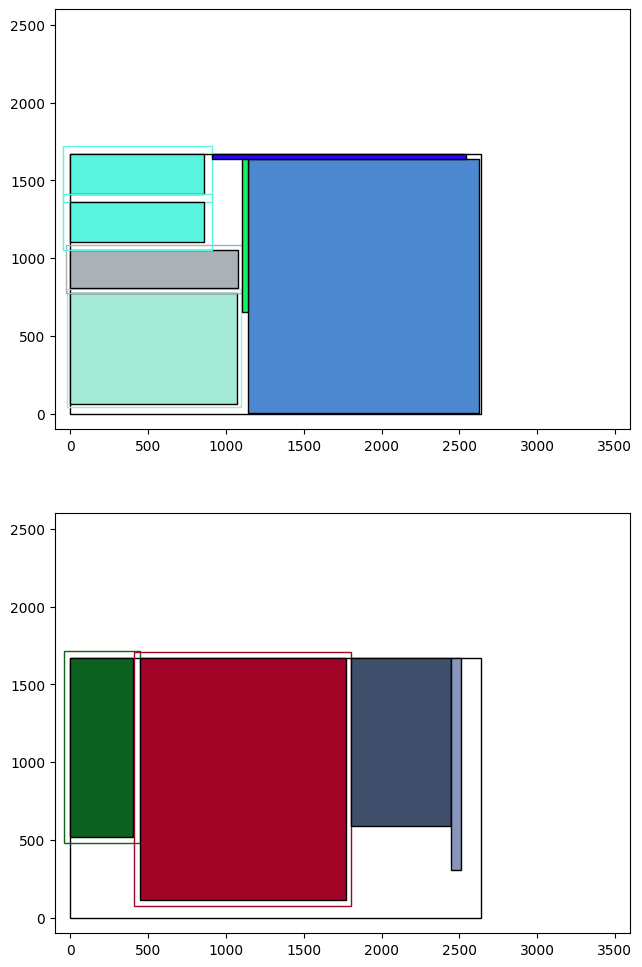
\includegraphics[width=1\columnwidth]{tesi/output} 
    \caption{Esempio nest di una soluzione}
\end{figure}




% \intro{Breve introduzione al capitolo}\\

% \section{Tecnologie e strumenti}
% \label{sec:tecnologie-strumenti}

% Di seguito viene data una panoramica delle tecnologie e strumenti utilizzati.

% \subsection*{Tecnologia 1}
% Descrizione Tecnologia 1.

% \subsection*{Tecnologia 2}
% Descrizione Tecnologia 2

% \section{Ciclo di vita del software}
% \label{sec:ciclo-vita-software}

% \section{Progettazione}
% \label{sec:progettazione}

% \subsubsection{Namespace 1} %**************************
% Descrizione namespace 1.

% \begin{namespacedesc}
%     \classdesc{Classe 1}{Descrizione classe 1}
%     \classdesc{Classe 2}{Descrizione classe 2}
% \end{namespacedesc}


% \section{Design Pattern utilizzati}

% \section{Codifica}
